\subsection*{Ejercicio 6}

\ejercicio{Retome el ejercicio de ordenación mediante el algoritmo de
  la burbuja. Ahora replique dicho ejercicio pero previamente deberá
  compilar el programa indicándole al compilador que optimice el
  código.Compare las curvas de eficiencia empírica para ver cómo
  mejora esto la eficiencia del programa.}

\begin{flushleft}
  Hemos compilado el programa indicado de dos maneras distintas:

  \[
    \text{g++ -O3 ordenacion.cpp -o burbuja}
  \]\[
        \text{g++ odernacion.cpp -o optimizado}
  \]
  
  Comprobamos al representar la nube de datos como se reduce de manera
  considerable el tiempo de ejecución de la version
  \textit{optimizada} respecto de la \textit{no optimizada}. Ambas curvas se ajustan a una curva del tipo $ax^2 +bx + c$
\end{flushleft}

\begin{figure}[H]
  \caption{Algoritmo bubble sort optimizado por el compilador}
  \centering
    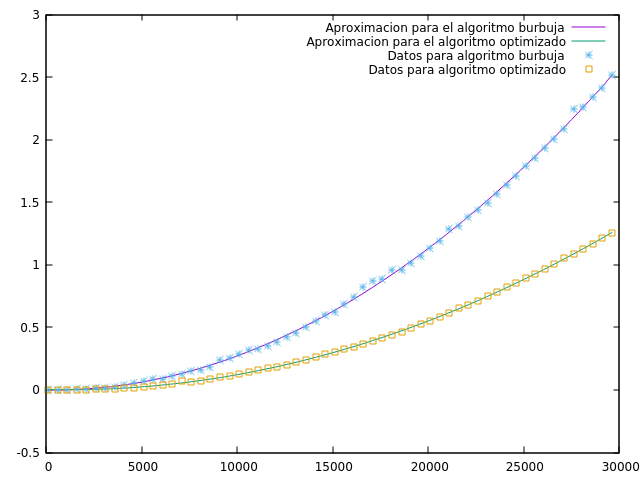
\includegraphics[width=0.7\textwidth]{ejer6/comparacion.png}
\end{figure}
